\documentclass[11pt,a4paper]{article}

\usepackage[utf8]{inputenc}
\usepackage[T1]{fontenc}
\usepackage[margin=2.3cm]{geometry}
\usepackage{amsmath}
\usepackage{graphicx}
\usepackage{booktabs}
\usepackage{float}
\usepackage{caption}
\usepackage{subcaption}
\usepackage{xcolor}
\usepackage[colorlinks=true,linkcolor=black,urlcolor=blue,citecolor=black]{hyperref}

% figures: "figures/" on Overleaf, "../reports/figures/" when compiled inside the repository
\graphicspath{{figures/}{../reports/figures/}}
\emergencystretch=3em  % lets long code words wrap without going into the margin

\title{Pay-Equity Audit with Supervised Learning\\[4pt]
\large A reference pay model to detect unexplained gaps by sex and race}
\author{Thomas Pasquier-Guillard, Lélia Hervy, Robin Cacarié\\[2pt]
\small Supervised Learning \& Model Engineering, Ilana Sebag, Albert School}
\date{October 2026}

\begin{document}
\maketitle

\noindent\textbf{Dataset:} Adult / Census Income, OpenML \texttt{adult} version 2 (R. Kohavi and B. Becker, 1996).\\
\textbf{Code:} \url{https://github.com/rcacarie-png/Adult-Income-Prediction}

\begin{abstract}
We take the role of a government agency that checks whether pay is fair with respect to sex and race, under the principle of equal pay for equal work. We train a reference pay model that predicts the probability of earning more than \$50K from job-related factors only, and never sees sex, race, national origin or their proxies. The audit then compares, for each group, the actual share of high earners with the share expected from its qualifications. The final model is a tuned LightGBM with isotonic calibration (test ROC-AUC 0.893, average precision 0.777, expected calibration error 0.009). On the untouched test set, women earn more than \$50K 5.4 points less often than their profiles predict (95\% CI $-6.3$ to $-4.6$), and Black employees 3.4 points less often ($-4.9$ to $-1.9$). A model trained on all columns is more accurate but hides these gaps entirely, which is why removing protected attributes is the right mitigation for this use case.
\end{abstract}

\section{Problem framing}

\paragraph{Business question.} A pay-equity regulator must decide which employers to investigate. Comparing the raw share of high earners between men and women is not enough: groups may differ in education, occupation or working time, which legitimately affect pay. The question is therefore: do people with the same job-related profile have the same chance of earning more than \$50K, whatever their sex or race?

\paragraph{Approach.} We learn $p(\text{income} > 50\text{K} \mid \text{job-related factors})$ on the population. For a group $g$ of size $n_g$, with actual labels $y_i$ and calibrated probabilities $\hat p_i$, we define
\[
\text{gap}_g = \frac{1}{n_g}\sum_{i \in g} y_i \;-\; \frac{1}{n_g}\sum_{i \in g} \hat p_i ,
\]
that is, the group's actual rate of high earners minus its expected rate. A significantly negative gap means the group earns less than its qualifications predict: a reason to open an investigation, not a proof of discrimination. This framing has three methodological consequences that structure the whole project:
\begin{enumerate}
\item Protected attributes and their proxies must not be inputs, otherwise the model learns the discrimination and the expected rate already contains it.
\item Probabilities must be calibrated, because the expected rate is an average of probabilities: inflated probabilities would make every group look underpaid.
\item Ranking quality matters (ROC-AUC, average precision), because the expected rate must follow the real differences in qualifications.
\end{enumerate}
Individual employees whose profile makes $>$\$50K more likely than not but who earn less are additionally flagged as potentially underpaid, for inspectors to review.

\section{Data and exploratory analysis}

\paragraph{Overview.} The 1994 US census extract contains 48,842 people, 6 numeric and 8 categorical columns. 23.9\% earn more than \$50K: the classes are imbalanced, and a model that always predicts ``$\leq$50K'' reaches 76.1\% accuracy with zero recall, so accuracy is not a useful metric here. Missing values concern only \texttt{workclass} (5.7\%), \texttt{occupation} (5.8\%, almost always together with \texttt{workclass}) and \texttt{native-country} (1.8\%). Missingness is informative: only 9.5\% of people with an unknown occupation earn $>$50K, against 24.8\% otherwise. We therefore encode it as an explicit ``Missing'' category instead of imputing the most frequent value. \texttt{capital-gain} and \texttt{capital-loss} are zero for 91.7\% and 95.3\% of people, with a long tail (maximum 99,999).

\paragraph{Sensitive attributes.} The raw gaps are large: 30.4\% of men earn $>$50K against 10.9\% of women; 25.4\% of White people against 12.1\% of Black people. Table~\ref{tab:gap} shows that the sex gap remains between people with the same education or the same occupation: legitimate factors do not explain it, which motivates the audit.

\begin{table}[H]
\centering
\caption{Share earning $>$\$50K by sex, within the same education level or occupation (full data).}
\label{tab:gap}
\begin{tabular}{lrr@{\hspace{1.5cm}}lrr}
\toprule
Education & Women & Men & Occupation & Women & Men \\
\midrule
High-school graduate (9) & 6.5\% & 20.3\% & Adm-clerical & 8.2\% & 24.9\% \\
Some college (10) & 7.0\% & 26.4\% & Exec-managerial & 24.1\% & 57.3\% \\
Bachelors (13) & 21.0\% & 50.3\% & Prof-specialty & 26.0\% & 56.0\% \\
Masters (14) & 34.3\% & 64.5\% & Sales & 6.9\% & 37.7\% \\
\bottomrule
\end{tabular}
\end{table}

\paragraph{Choice of columns.} Table~\ref{tab:columns} summarises which columns the reference model may use. Beyond the protected attributes, \texttt{relationship} is an almost perfect proxy for sex (19,715 of the 19,716 ``Husband'' are men, 2,328 of the 2,331 ``Wife'' are women), and marital status is not a job-related factor, so both are excluded even though they are among the strongest predictors. \texttt{fnlwgt} is a census sampling weight with no relationship to income ($>$50K rate between 21.6\% and 25.4\% across its deciles), and \texttt{education} duplicates \texttt{education-num} exactly.

\begin{table}[H]
\centering
\caption{Column decisions for the reference pay model.}
\label{tab:columns}
\begin{tabular}{p{5.2cm}p{2.2cm}p{6.8cm}}
\toprule
Column(s) & Decision & Reason \\
\midrule
sex, race, native-country & excluded & protected attributes, used only to group the audit \\
relationship, marital-status & excluded & proxy for sex / not a job-related factor \\
fnlwgt & excluded & census sampling weight, no link with income \\
education & excluded & exact duplicate of education-num \\
age, education-num, workclass, occupation, hours-per-week & kept & legitimate pay factors: experience, qualification, job, working time \\
capital-gain, capital-loss & kept, tested & investment income, part of the target (see the leakage audit) \\
\bottomrule
\end{tabular}
\end{table}

\paragraph{Leakage audit.} Every kept column is known at prediction time, with one caveat: the target is total income, which includes capital gains. \texttt{capital-gain} is therefore a partial target leak. We keep it, because ignoring investment income would attribute it to the employer, and we verify in Section~\ref{sec:robust} that the conclusions do not depend on it. The census has no dates and no person identifier, so there is no temporal leakage to audit and group leakage cannot be checked; the 52 duplicated rows are plausible different people with identical profiles.

\paragraph{Split.} We use a stratified 60/20/20 split (\texttt{random\_state=42}): 29,304 training, 9,769 validation and 9,769 test people, each with a 23.9\% positive rate. The training set is used for fitting and cross-validation, the validation set for model choice, calibration choice and threshold, and the test set is opened once, at the end, for the final evaluation and the audit. We keep a separate validation set, rather than only cross-validation on 80\% of the data as in the course protocol, because the calibration and the threshold must be chosen on data the model was not trained on, without touching the test set.

\section{Methodology}

\subsection{Feature engineering and pipeline}

A custom scikit-learn transformer, \texttt{AdultFeatureEngineer}, drops the excluded columns and adds five features (Table~\ref{tab:features}). Numeric columns are then imputed with the median and standardised; categorical columns are imputed with ``Missing'' and one-hot encoded, with rare categories ($<$0.5\%) grouped together and unknown categories handled at prediction time. All steps and the model are wrapped in a single \texttt{Pipeline}, so every preprocessing step is fitted on the training data (or the training folds) only, and the excluded columns can never reach the model, even at serving time.

\begin{table}[H]
\centering
\caption{Engineered features and their signal on the training set ($>$50K rate).}
\label{tab:features}
\begin{tabular}{llp{7.5cm}}
\toprule
Feature & Definition & Justification and signal \\
\midrule
capital\_net & gain $-$ loss & net investment result in one number \\
has\_capital & gain $>0$ or loss $>0$ & owning investments: 57.5\% vs 18.9\% \\
log\_capital\_gain & $\log(1 + \text{gain})$ & tames the long tail for the linear model \\
works\_overtime & hours $>$ 40 & 39.7\% vs 17.2\% \\
is\_part\_time & hours $<$ 35 & 7.2\% vs 27.4\%; 27.6\% of women vs 11.9\% of men \\
\bottomrule
\end{tabular}
\end{table}

The working-time features matter for the audit: women work part-time much more often, a legitimate reason for lower annual income that the model must account for.

\subsection{Metrics and class imbalance}

We report precision, recall and F1 at the decision threshold, and two threshold-free ranking metrics: ROC-AUC and average precision (AP, the area under the precision-recall curve, called \texttt{pr\_auc} in our code; a random model scores the prevalence, 0.24). AP is our main selection metric, since it focuses on the rare class.

On the Logistic Regression baseline, we compared three remedies (Table~\ref{tab:imbalance}). All three give the same trade-off: recall rises from 0.43 to about 0.76, precision falls from 0.74 to about 0.51, F1 improves, and ROC-AUC and AP do not move. The remedies shift the operating point (they are close to lowering the threshold), they do not improve the ranking. We keep class weights (\texttt{class\_weight="balanced"}): same result, all real data is kept (undersampling discards two thirds of the majority class), no synthetic people (SMOTE interpolates one-hot columns into unrealistic profiles), and the same parameter exists for all three models. Resampling, when used, is applied inside an \texttt{imblearn} pipeline, during fit only.

\begin{table}[H]
\centering
\caption{Class-imbalance remedies on Logistic Regression (validation set, threshold 0.5).}
\label{tab:imbalance}
\begin{tabular}{lrrrrrr}
\toprule
Remedy & Precision & Recall & F1 & ROC-AUC & AP & Fit time (s) \\
\midrule
None & 0.744 & 0.431 & 0.546 & 0.853 & 0.692 & 0.5 \\
Class weights & 0.508 & 0.756 & 0.607 & 0.854 & 0.691 & 0.5 \\
Random undersampling & 0.510 & 0.760 & 0.611 & 0.854 & 0.689 & 0.2 \\
SMOTE & 0.510 & 0.757 & 0.609 & 0.854 & 0.692 & 1.0 \\
\bottomrule
\end{tabular}
\end{table}

We treat the class weight as fixed rather than as a hyperparameter: it did not change the ranking, and the precision/recall trade-off is controlled later by the threshold. Its side effect on the probabilities is corrected by calibration (Section~\ref{sec:calib}). In the end, after calibration and with the 0.5 threshold, the class weights no longer raise recall (0.50 on the test set): they never improved the ranking, and the precision/recall trade-off is set by the threshold.

\subsection{Models, tuning and experiment tracking}

We compare Logistic Regression (linear, interpretable: the baseline the course asks us to start with), Random Forest (bagged deep trees, captures interactions) and LightGBM (gradient boosting, the fast histogram-based implementation seen in class, preferred to scikit-learn's slower GradientBoosting), all with class weights and the same pipeline. Hyperparameters are tuned with Optuna (TPE sampler, seed 42): 15 trials for Logistic Regression and the Random Forest, 30 for LightGBM. Each trial is scored by 5-fold stratified cross-validation on the training set (\texttt{scoring="average\_precision"}), refitting the whole pipeline in each fold; the validation set is never used during the search, so the selection does not overfit it. Search spaces cover the complexity parameters of each model (Appendix~\ref{app:search}).

Every run is logged in MLflow (experiment \texttt{adult-pay-equity}, SQLite backend, committed in the repository): parameters, metrics, confusion matrices and fitted pipelines for the imbalance and model comparisons; one parent run per model with one nested child run per Optuna trial (parameters, CV mean and standard deviation, the five fold scores, run time) and the optimisation history; and a final run with the test metrics, the audit tables and the calibrated model. Runs are tagged by stage (imbalance, models, tuning, tuned, final\_test).

\section{Results}

\subsection{Modelling progression}

\begin{table}[H]
\centering
\caption{Model comparison. CV: 5-fold AP on the training set (mean $\pm$ std). Validation metrics at threshold 0.5, before calibration.}
\label{tab:models}
\small
\begin{tabular}{llrrrrrr}
\toprule
Model & Version & CV AP & Val. AP & Val. ROC-AUC & Precision & Recall & F1 \\
\midrule
Logistic Regression & default & $0.684 \pm 0.005$ & 0.691 & 0.854 & 0.508 & 0.756 & 0.607 \\
 & tuned & $0.684 \pm 0.005$ & 0.692 & 0.854 & 0.508 & 0.756 & 0.607 \\
Random Forest & default & $0.738 \pm 0.010$ & 0.752 & 0.880 & 0.540 & 0.771 & 0.635 \\
 & tuned & $0.738 \pm 0.011$ & 0.756 & 0.881 & 0.522 & 0.797 & 0.631 \\
LightGBM & default & $0.761 \pm 0.008$ & 0.772 & 0.890 & 0.544 & 0.804 & 0.649 \\
 & tuned & $0.764 \pm 0.010$ & 0.776 & 0.893 & 0.544 & 0.804 & 0.649 \\
\bottomrule
\end{tabular}
\end{table}

\paragraph{What each step bought.} Moving from Logistic Regression to the Random Forest brings the largest gain (AP $+0.06$, ROC-AUC $+0.025$): trees capture interactions that a linear score cannot, for example the return on education depends on occupation and age. LightGBM adds a further gain (AP $+0.02$) with the best recall, and both tree models train in a few seconds. Both tree models overfit mildly (train vs validation ROC-AUC: 0.914 vs 0.880 for the forest, 0.911 vs 0.890 for LightGBM); Logistic Regression does not.

\paragraph{What tuning bought.} Very little: AP rises by $+0.005$ for LightGBM, $+0.004$ for the forest and about 0 for Logistic Regression on validation, which is smaller than the cross-validation standard deviation. Tuning mostly reduced overfitting: training AP drops from 0.802 to 0.788 for LightGBM and from 0.806 to 0.796 for the forest while validation AP slightly rises. The best LightGBM uses many small steps (600 trees, learning rate 0.023) and moderate trees (22 leaves, 51\% of features per tree). The CV and validation rankings agree, and validation scores are about 0.01 above the CV scores for every model (tuned or not), so the selection over many trials did not produce an optimistic estimate. The model family mattered more than the hyperparameters.

\paragraph{Final choice.} We select the tuned LightGBM: best validation AP and ROC-AUC, consistent CV and validation results, and exact, fast SHAP explanations for trees.

\paragraph{Reproducibility.} All numbers come from the MLflow history committed in the repository (run with \texttt{python -m src.part5\_serving}). Every random step uses \texttt{random\_state=42}; only the Random Forest varies very slightly between machines (multi-threaded trees), which changes none of the conclusions.


\subsection{Explainability}

We explain the final model with SHAP (\texttt{TreeExplainer}, log-odds scale) on 2,000 validation people. Globally (Figure~\ref{fig:shap}a), the most important features are age (mean $|$SHAP$|$ 1.09), education (0.47), capital gain and \texttt{capital\_net} (0.29, 0.22), hours per week (0.20) and occupations (Other-service, Exec-managerial, Adm-clerical). Four of the five engineered features are in the top 15. These are exactly the factors that pay should legitimately depend on: experience, qualification, working time, investment income and type of job. The directions make sense: older, more educated people working longer hours are pushed towards $>$50K; service and clerical occupations push down. SHAP describes what the model uses, not what causes income.

Locally, the instructive cases are the model's mistakes (Figure~\ref{fig:shap}b and Appendix~\ref{app:figures}). The ``missed high earner'' is a 46-year-old woman with an 11th-grade education working 35 hours a week in Other-service: every job-related factor points to $\leq$50K, her high income is genuinely unusual for her profile. The ``false alarm'' is a self-employed 50-year-old with a professional degree whom everything predicts above \$50K: exactly what a ``potentially underpaid'' flag looks like, but with no employer to blame, which shows that flags are starting points for an inspector, not conclusions.

\begin{figure}[H]
\centering
\begin{subfigure}{0.49\textwidth}
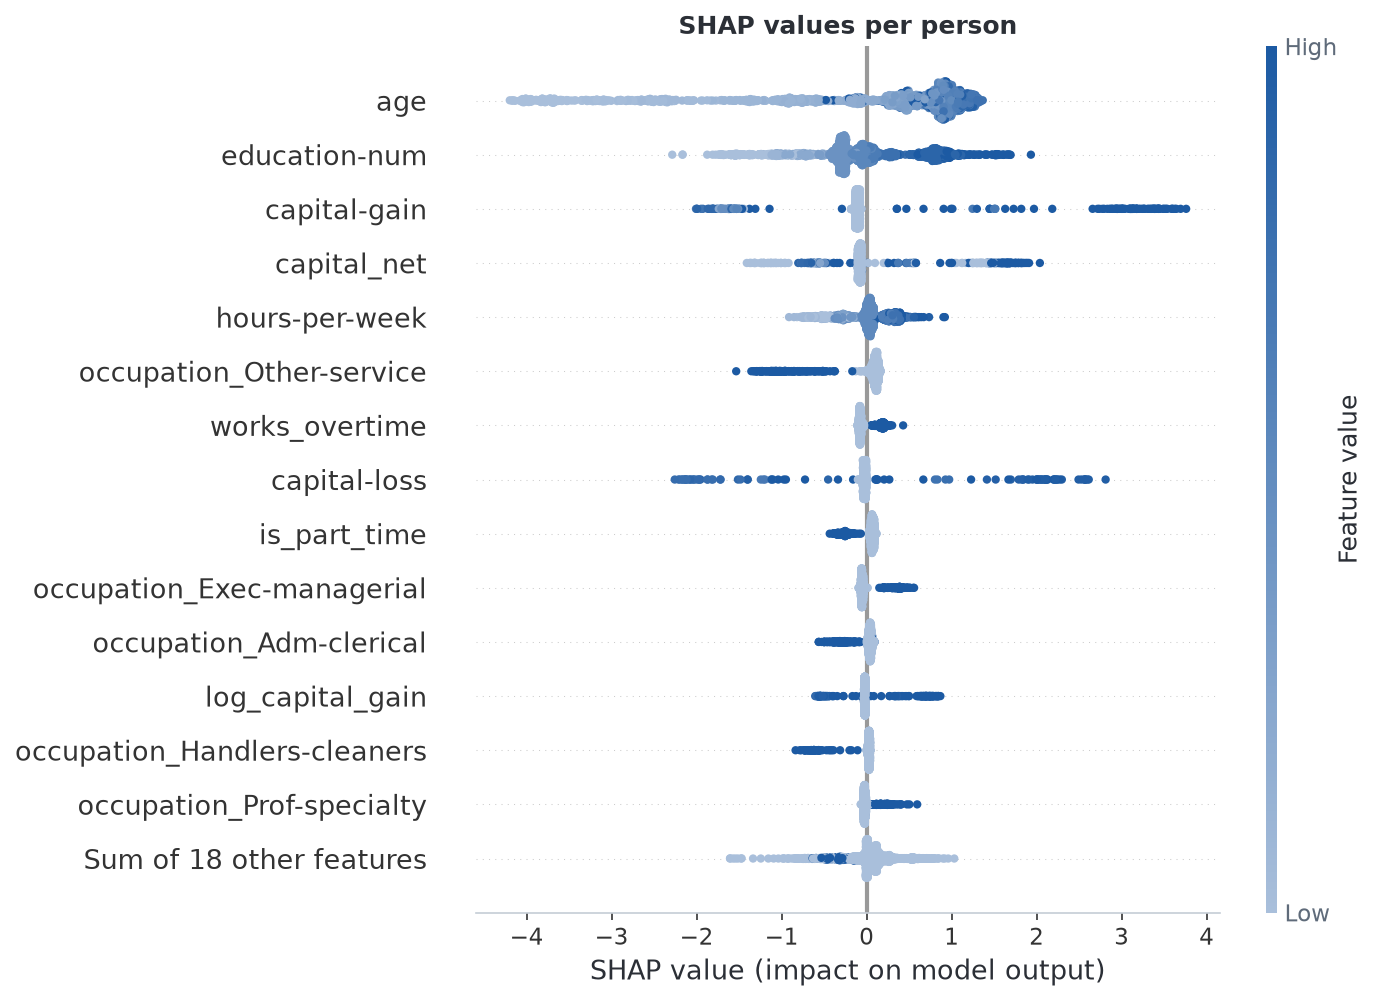
\includegraphics[width=\textwidth]{part4_02.png}
\caption{Global: SHAP beeswarm (navy = high feature value).}
\end{subfigure}
\hfill
\begin{subfigure}{0.49\textwidth}
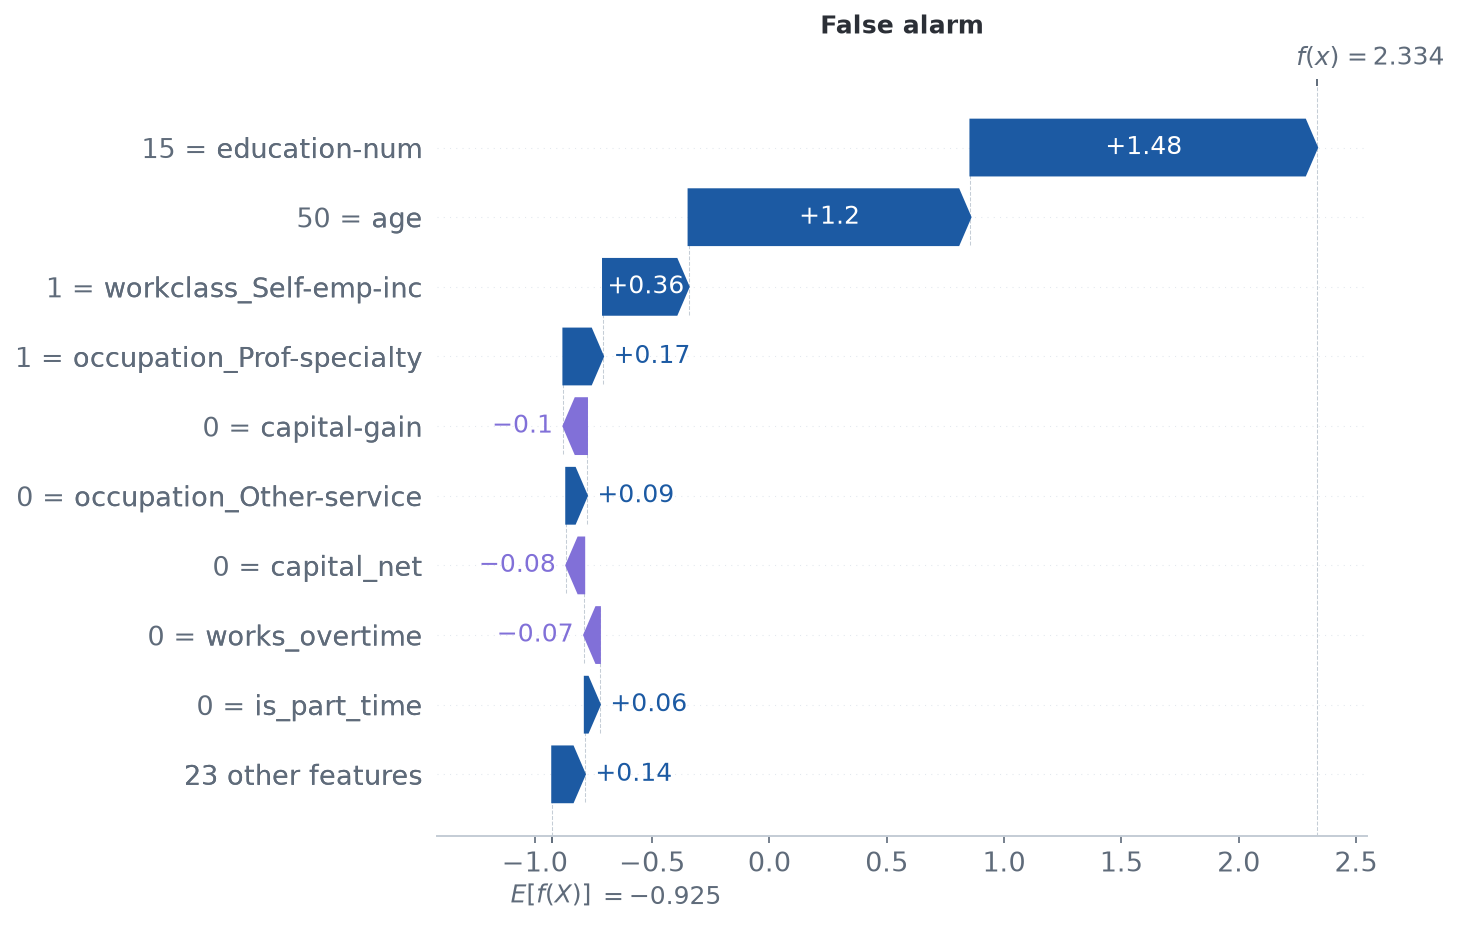
\includegraphics[width=\textwidth]{part4_06.png}
\caption{Local: the ``false alarm'' (really $\leq$50K, predicted 0.91).}
\end{subfigure}
\caption{SHAP explanations of the final LightGBM.}
\label{fig:shap}
\end{figure}

\subsection{Calibration diagnostics}
\label{sec:calib}

\begin{table}[H]
\centering
\caption{Calibration of the final model (validation set). ECE with 10 equal-width bins.}
\label{tab:calib}
\small
\begin{tabular}{lrrrrr}
\toprule
Probabilities & Brier score & ECE & Mean predicted & Observed rate & AP \\
\midrule
Raw (class-weighted LightGBM) & 0.132 & 0.135 & 0.374 & 0.239 & 0.776 \\
Sigmoid calibration & 0.105 & 0.031 & 0.236 & 0.239 & 0.776 \\
Isotonic calibration & 0.103 & 0.010 & 0.236 & 0.239 & 0.775 \\
\bottomrule
\end{tabular}
\end{table}

The raw model is over-confident towards $>$50K: it predicts 37\% on average while the true rate is 24\%, and its reliability curve lies below the diagonal (Figure~\ref{fig:calib}a). This is the expected side effect of class weights, which make each positive count about three times more during training. We would not trust these probabilities as they are: the audit would declare almost every group underpaid. We recalibrate with \texttt{CalibratedClassifierCV(cv=5)}, which learns the mapping on out-of-fold predictions of the training set, so neither the validation nor the test set is used. Isotonic regression clearly beats the sigmoid (ECE three times lower), and with 29,000 training people it has enough data not to overfit, so we keep it; AP is unchanged since calibration preserves the ranking. Bin counts (Appendix~\ref{app:figures}) show that the low-probability region, which drives the group averages, is estimated on thousands of people, while bins between 0.5 and 0.9 contain only 90 to 460 people; there the model is, if anything, slightly cautious (observed 0.75 for 0.65 predicted).

\begin{figure}[H]
\centering
\begin{subfigure}{0.45\textwidth}
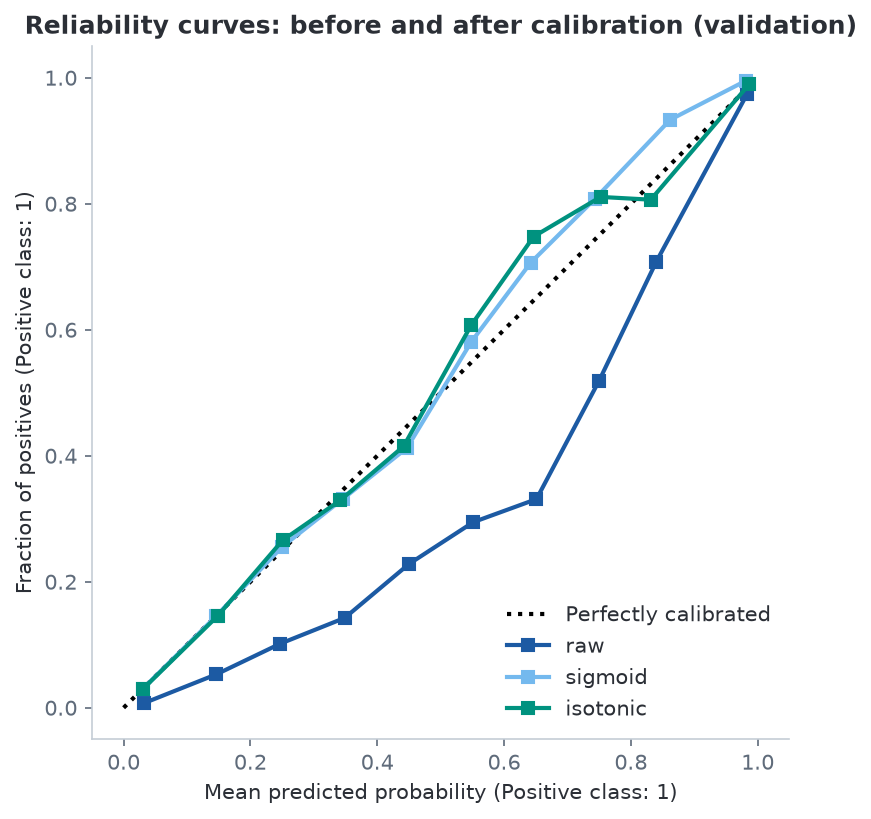
\includegraphics[width=\textwidth]{part4_08.png}
\caption{Reliability curves (validation).}
\end{subfigure}
\hfill
\begin{subfigure}{0.53\textwidth}
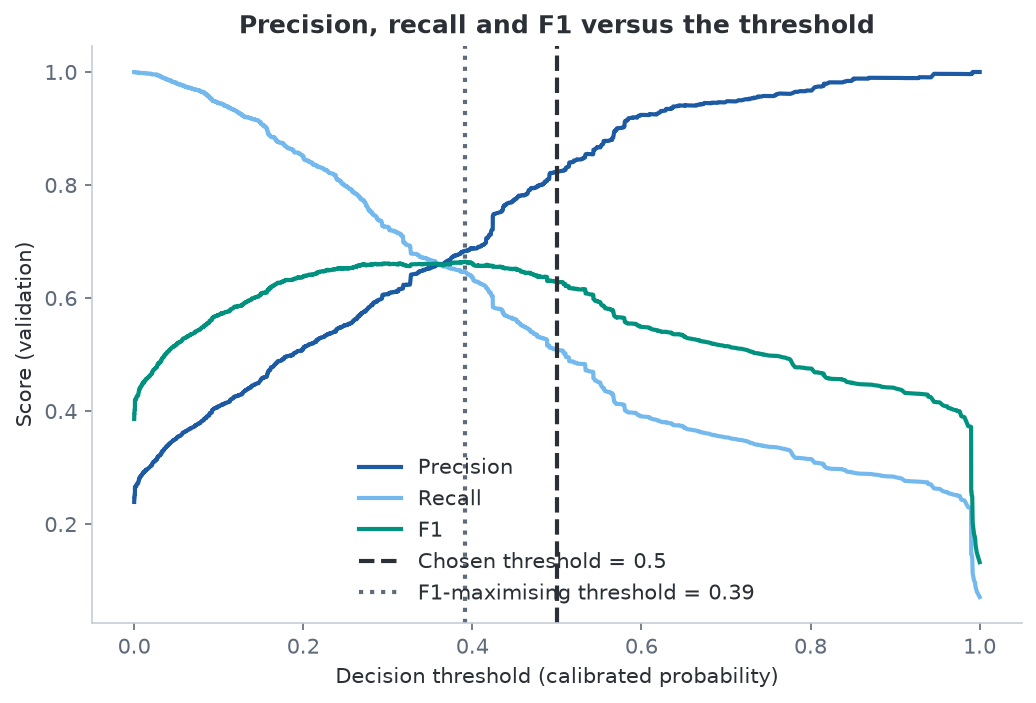
\includegraphics[width=\textwidth]{part4_10.png}
\caption{Precision, recall and F1 vs threshold (calibrated).}
\end{subfigure}
\caption{Calibration and choice of the decision threshold.}
\label{fig:calib}
\end{figure}

\subsection{Decision rule and final test}

Individual flags use the calibrated probability with a threshold of 0.5 (``more likely than not''). Since a flag may trigger an inspection and inspectors are limited, precision matters more than recall: at 0.5, 82\% of people expected to earn $>$50K really do (recall 0.51), whereas the F1-optimal threshold (0.39) would trade precision down to 0.68 for a recall of 0.65. The group audit does not depend on the threshold, as it uses the probabilities directly.

\begin{table}[H]
\centering
\caption{Final model (tuned LightGBM, isotonic calibration, threshold 0.5): validation vs untouched test set.}
\label{tab:final}
\begin{tabular}{lrrrrrrrr}
\toprule
Set & Accuracy & Precision & Recall & F1 & ROC-AUC & AP & Brier & ECE \\
\midrule
Validation & 0.857 & 0.824 & 0.509 & 0.629 & 0.893 & 0.775 & 0.103 & 0.010 \\
Test & 0.854 & 0.818 & 0.501 & 0.621 & 0.893 & 0.777 & 0.103 & 0.009 \\
\bottomrule
\end{tabular}
\end{table}

Test and validation results are nearly identical: the choices made on validation did not overfit it, and these are honest estimates for new people from the same population. Following the course protocol strictly would refit on train + validation before testing; we did not, because the validation set was used to choose the calibration and the threshold, and refitting would change the model after those choices for a small gain from 20\% more data.

\section{Fairness and pay-equity audit}

Two questions must be kept apart, each with its own fairness definition. Is the pay fair? Our definition is ``equal pay for equal work'' (conditional parity): people with the same job-related profile should have the same probability of earning more than \$50K, whatever their group; the unexplained gap measures how far each group is from it. Is our model fair? It must give the same output to the same profile, whatever the person's group. Demographic parity, equal opportunity and equalized odds are reported below for completeness. All results are on the test set.

\subsection{Classic fairness metrics of the model}

\begin{table}[H]
\centering
\caption{Group metrics of the final model by sex (test set). Gaps (0 = equal): demographic parity 0.103, equal opportunity 0.042, equalized odds 0.042.}
\label{tab:fair}
\begin{tabular}{lrrrrrr}
\toprule
Sex & n & Base rate & Selection rate & TPR & FPR & Precision \\
\midrule
Women & 3,259 & 0.111 & 0.078 & 0.465 & 0.029 & 0.664 \\
Men & 6,510 & 0.304 & 0.181 & 0.507 & 0.039 & 0.851 \\
\bottomrule
\end{tabular}
\end{table}

Demographic parity (same share predicted $>$50K) is not satisfied, purely because job-related profiles differ (hours, part-time work, occupations); the model's selection gap (10 points) is much smaller than the real gap (19 points). Equal opportunity and equalized odds are nearly satisfied: true and false positive rates differ by at most 4 points. The telling number is precision: among people the model expects to earn $>$50K, 85\% of men do, but only 66\% of women. For our model, a false positive is a person whose qualifications predict a high income but who does not receive it: a lower precision for women is evidence about the pay, not a defect of the model. By race, the largest gaps (0.12) come from the 96-person Amer-Indian-Eskimo group and are not reliable; Black employees have a higher precision (0.86) than White employees (0.82).

\subsection{Pay-equity audit}

\begin{table}[H]
\centering
\caption{Pay-equity audit on the test set. Gap = actual $-$ expected rate, in percentage points, with a 95\% bootstrap CI (1,000 resamples). Underpaid: share of employees expected to earn $>$50K who do not. Groups under 100 people are not interpreted.}
\label{tab:audit}
\begin{tabular}{lrrrcr}
\toprule
Group & n & Actual & Expected & Gap [95\% CI] & Underpaid \\
\midrule
Women & 3,259 & 11.1\% & 16.5\% & $-5.4$ [$-6.3$, $-4.6$] & 34\% \\
Men & 6,510 & 30.4\% & 27.1\% & $+3.3$ [$+2.4$, $+4.2$] & 15\% \\
Black & 968 & 13.3\% & 16.7\% & $-3.4$ [$-4.9$, $-1.9$] & 14\% \\
White & 8,312 & 25.3\% & 24.4\% & $+0.9$ [$+0.2$, $+1.6$] & 18\% \\
Asian-Pac-Islander & 311 & 26.4\% & 25.4\% & $+1.0$ [$-2.9$, $+5.0$] & 29\% \\
Amer-Indian-Eskimo & 96 & 13.5\% & 16.4\% & \multicolumn{2}{c}{too small to conclude} \\
Other & 82 & 12.2\% & 14.8\% & \multicolumn{2}{c}{too small to conclude} \\
\bottomrule
\end{tabular}
\end{table}

Women earn more than \$50K 5.4 points less often than their job-related profiles predict, and a third of the women expected to earn $>$50K do not, against 15\% of men. Black employees earn 3.4 points less than expected; for them the gap is spread over moderate probabilities rather than concentrated among the individuals the model expects to be high earners (only 14\% of them are flagged). Both gaps are significant. White employees are slightly above expectation (significant only because the group is large); the Asian-Pacific-Islander gap is not significant. Since the model is calibrated on the whole population, its expected rate matches the overall actual rate (overall gap +0.4 points), so group gaps partly offset each other: the positive gap for men is largely the counterpart of the negative gap for women.

\begin{figure}[H]
\centering
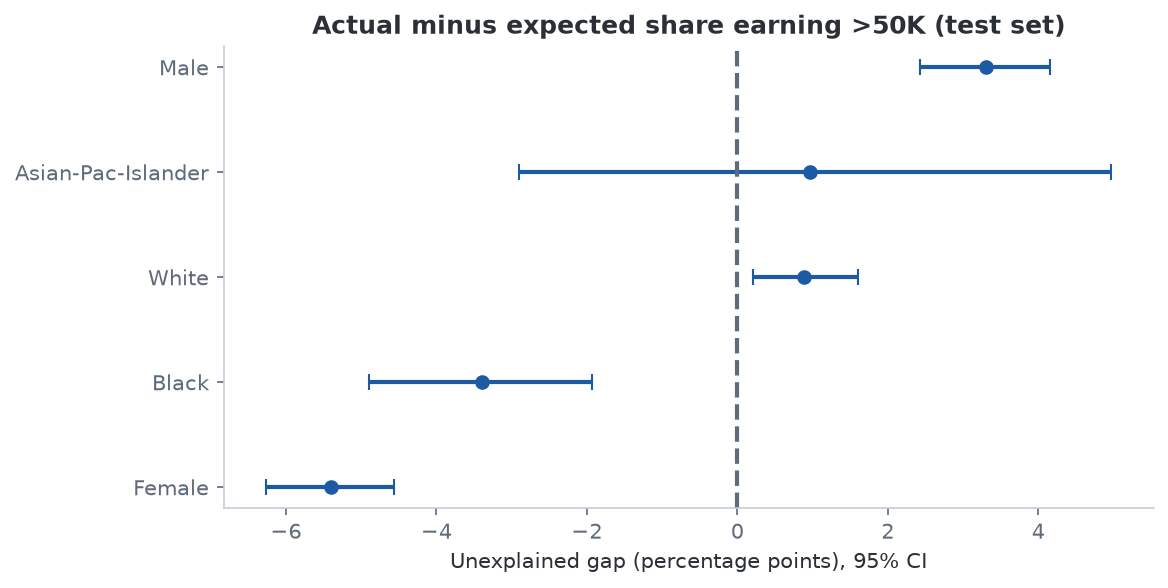
\includegraphics[width=0.75\textwidth]{part4_13.png}
\caption{Unexplained gap by group with 95\% bootstrap confidence intervals (test set, groups of at least 100 people).}
\end{figure}

\subsection{Mitigation: before / after}

Our mitigation is a pre-processing technique: removing the protected attributes and their proxies from the model's inputs. Removing them alone (``fairness through unawareness'') is known to be insufficient, because other inputs can partly rebuild them: the proxy check of Section~\ref{sec:robust} measures how much. To measure its effect, the ``before'' model uses the same tuned LightGBM, calibration and threshold, but is trained on all columns, including sex, race, national origin, marital status and relationship.

\begin{table}[H]
\centering
\caption{Before / after the mitigation, on the untouched test set.}
\label{tab:mitigation}
\begin{tabular}{lrr}
\toprule
 & Before: all columns & After: job-related only \\
\midrule
ROC-AUC / AP & 0.930 / 0.834 & 0.893 / 0.777 \\
F1 (threshold 0.5) & 0.721 & 0.621 \\
Demographic parity difference (sex) & 0.187 & 0.103 \\
Equalized odds difference (sex) & 0.114 & 0.042 \\
Unexplained gap, women & $+0.2$ pts & $-5.4$ pts \\
Unexplained gap, Black employees & $+1.1$ pts & $-3.4$ pts \\
\bottomrule
\end{tabular}
\end{table}

The mitigation costs predictive performance (ROC-AUC $-0.04$, F1 $-0.10$) but almost halves the demographic-parity gap and nearly divides the equalized-odds gap by three. Above all, it changes the audit: the ``before'' model is more accurate because it has learned the discrimination. It expects lower pay for women and Black employees, finds them paid exactly as expected, and would declare every employer fair. A reference model must describe what people should earn for their work, not what they do earn given their sex and race.

We rejected post-processing (for example fairlearn's \texttt{ThresholdOptimizer}). It equalises error rates with group-specific thresholds, which suits a model that decides about people (hiring, credit), but here the extra ``errors'' for women are the underpayment signal: equalising them would erase the evidence, and it would require sex and race at prediction time.

\subsection{Robustness checks}
\label{sec:robust}

\paragraph{Proxy check.} A classifier predicting sex from the model's inputs reaches ROC-AUC 0.79, mainly through occupation and hours. This is intended under ``equal pay for equal work'' (part-time work legitimately lowers annual income), but it means the gap only measures unequal pay for comparable jobs: discrimination in access to well-paid occupations is ``explained'' by occupation and remains invisible. Our gaps are therefore a lower bound.

\paragraph{Sensitivity to the capital columns.} Retraining without \texttt{capital-gain}, \texttt{capital-loss} and their engineered features lowers ROC-AUC from 0.893 to 0.846, but the conclusions hold and the gaps become slightly larger: $-6.6$ pts for women (CI $-7.6$ to $-5.5$) and $-3.8$ pts for Black employees ($-5.6$ to $-2.0$), because investment income is more frequent among men. Keeping these columns is the conservative choice for employers.

\section{Serving}

The calibrated pipeline is exported with cloudpickle together with its settings, and served by a FastAPI application (\texttt{serving/audit\_api.py}) with Pydantic input validation. \texttt{GET /health} checks the service; \texttt{POST /predict} returns each employee's expected probability; \texttt{POST /audit} takes a company's employee records and returns, per sex and race group, the actual and expected rates, the gap with its bootstrap CI, and the potentially underpaid employees. Tests with FastAPI's \texttt{TestClient} confirm that two employees with the same job profile but different sex and race receive exactly the same probability (0.652), and that invalid inputs (for example an age of 7) are rejected with HTTP 422. On a simulated company of 2,000 test-set employees, the API reports a significant gap for women ($-6.0$ pts, CI $-7.8$ to $-4.0$) and flags 52 potentially underpaid employees.

\section{Discussion and limitations}

\paragraph{What could invalidate the conclusions.}
\begin{itemize}
\item \textbf{Unexplained is not proven.} Factors absent from the data (seniority, exact job title, region, firm size, performance) could legitimately explain part of the gaps.
\item \textbf{The reference is the population.} The model learns the average pay of a population that includes the discrimination we audit, and occupation can itself reflect discrimination: both bias the gaps towards zero.
\item \textbf{The data.} The census describes individuals, not companies; the target is total income rather than salary, binarised at a coarse \$50K threshold; and the data dates from 1994. The method transfers, the size of the gaps does not.
\item \textbf{Small groups.} Two race groups have fewer than 100 test people; their gaps cannot be interpreted. Calibration was checked globally; checking it within each group would further strengthen the audit.
\end{itemize}

\paragraph{Conclusion.} A calibrated reference model trained on job-related factors only is an effective screening tool for a pay-equity regulator. On this data, it reveals significant unexplained gaps for women ($-5.4$ pts) and Black employees ($-3.4$ pts), robust to the removal of the leaky capital columns, that a model trained on all columns would completely hide. We recommend using it to prioritise investigations, with the gap and its confidence interval as the trigger and the individual flags as the starting point for inspectors.

\section*{Contribution statement}

\begin{table}[H]
\centering
\begin{tabular}{p{4.2cm}p{11cm}}
\toprule
Member & Contributions \\
\midrule
Lélia Hervy & Wrote most of the code: exploration, feature engineering, pipeline, imbalance comparison, model comparison, tuning, calibration, SHAP, fairness and pay-equity audit, API; merged the analysis into the final notebook and scripts; maintains the repository. \\
Thomas Pasquier-Guillard & Defined the research question (pay fairness with respect to sex and race, ``equal pay for equal work''); reviewed and modified the code. \\
Robin Cacarié & Proposed framing the project around a real problem (the pay-equity regulator); created the GitHub repository; reviewed and modified the code; prepared the slides for the final presentation. \\
\bottomrule
\end{tabular}
\end{table}

\noindent All members contributed to the report and the oral defense, and can explain every part of the project.

\paragraph{Use of AI assistants.} We used Claude (Anthropic) as a coding assistant to generate and explain code, check the consistency of results against the course material, and help draft this report. We reviewed, ran and modified all code ourselves, verified every number against our own runs, and discussed and validated every methodological choice as a team.

\section*{References}
\begin{itemize}
\item R. Kohavi. Scaling up the accuracy of naive-Bayes classifiers: a decision-tree hybrid. KDD, 1996. (Adult dataset)
\item F. Pedregosa et al. Scikit-learn: Machine learning in Python. JMLR 12, 2011.
\item G. Ke et al. LightGBM: A highly efficient gradient boosting decision tree. NeurIPS, 2017.
\item T. Akiba et al. Optuna: A next-generation hyperparameter optimization framework. KDD, 2019.
\item S. Lundberg and S.-I. Lee. A unified approach to interpreting model predictions. NeurIPS, 2017.
\item A. Niculescu-Mizil and R. Caruana. Predicting good probabilities with supervised learning. ICML, 2005.
\item M. Hardt, E. Price and N. Srebro. Equality of opportunity in supervised learning. NeurIPS, 2016.
\item H. Weerts et al. Fairlearn: Assessing and improving fairness of AI systems. JMLR 24, 2023.
\end{itemize}

\appendix

\section{Hyperparameter search spaces}
\label{app:search}

\begin{table}[H]
\centering
\small
\begin{tabular}{p{2.6cm}p{7.4cm}p{5.2cm}}
\toprule
Model & Search space & Best (CV AP) \\
\midrule
Logistic Regression & C in [$10^{-3}$, 100] (log) & C = 71 (0.684) \\
Random Forest & n\_estimators 100 to 400, max\_depth 5 to 30, min\_samples\_leaf 1 to 50 (log), max\_features in \{sqrt, 0.3, 0.5\} & 350 trees, depth 13, leaf 2, max\_features 0.5 (0.738) \\
LightGBM & n\_estimators 100 to 800, learning\_rate 0.01 to 0.2 (log), num\_leaves 8 to 128 (log), min\_child\_samples 5 to 100 (log), subsample 0.5 to 1, colsample\_bytree 0.5 to 1, reg\_lambda $10^{-3}$ to 10 (log) & 600 trees, lr 0.023, 22 leaves, min child 5, subsample 0.89, colsample 0.51, $\lambda$ 0.049 (0.764) \\
\bottomrule
\end{tabular}
\caption*{All models use \texttt{class\_weight="balanced"} and \texttt{random\_state=42}.}
\end{table}

\section{Additional figures}
\label{app:figures}

\begin{figure}[H]
\centering
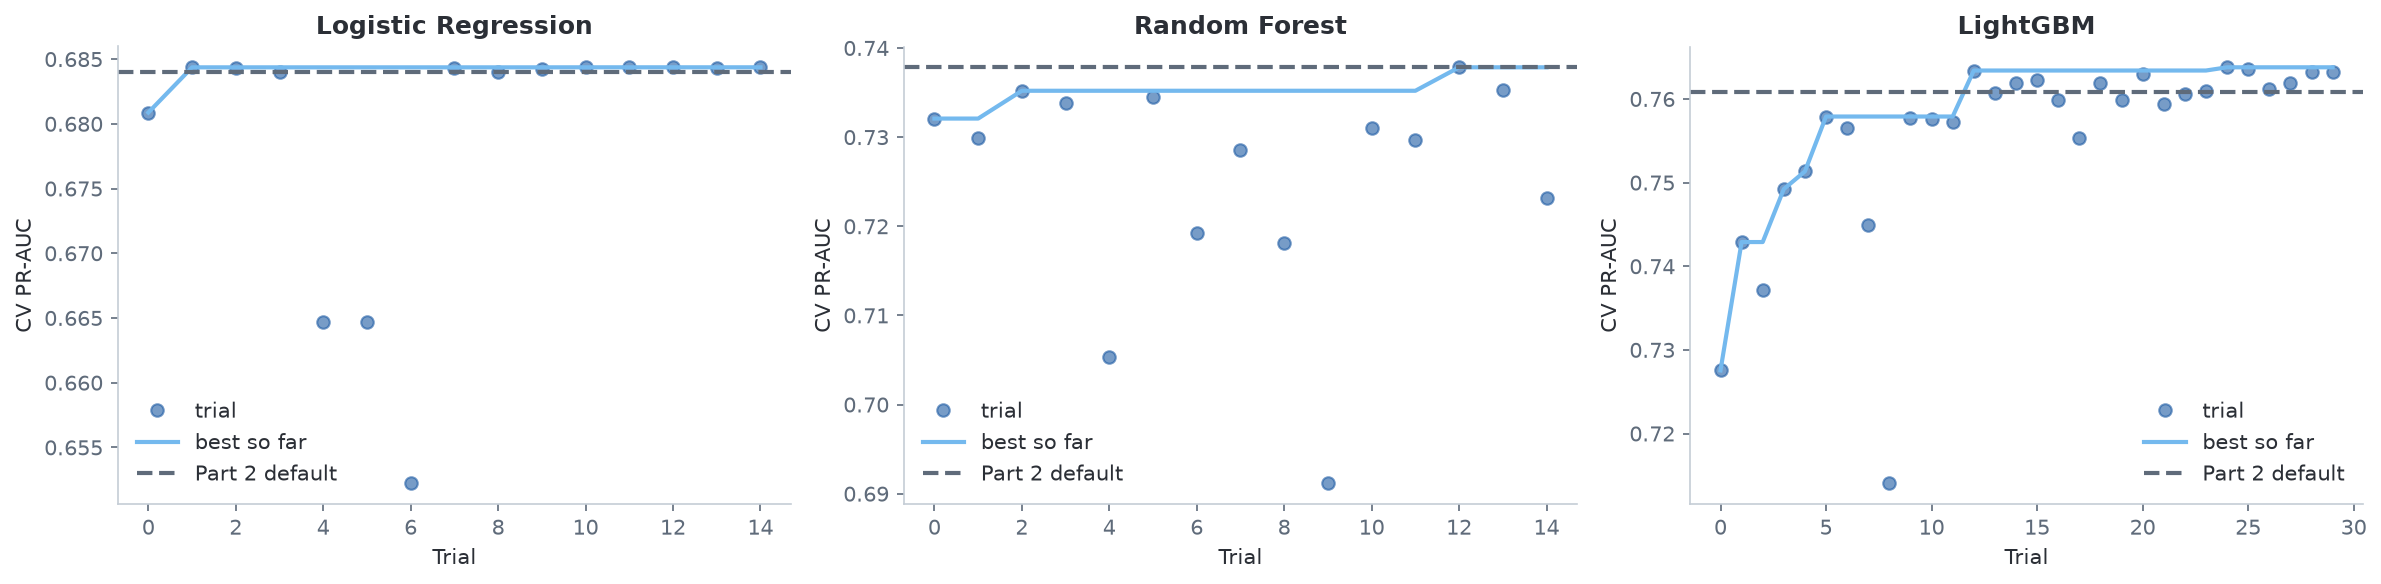
\includegraphics[width=\textwidth]{part3_01.png}
\caption{Optuna search (Section 4.1): CV average precision of each trial, best so far, and the untuned model (dashed).}
\end{figure}

\begin{figure}[H]
\centering
\begin{subfigure}{0.49\textwidth}
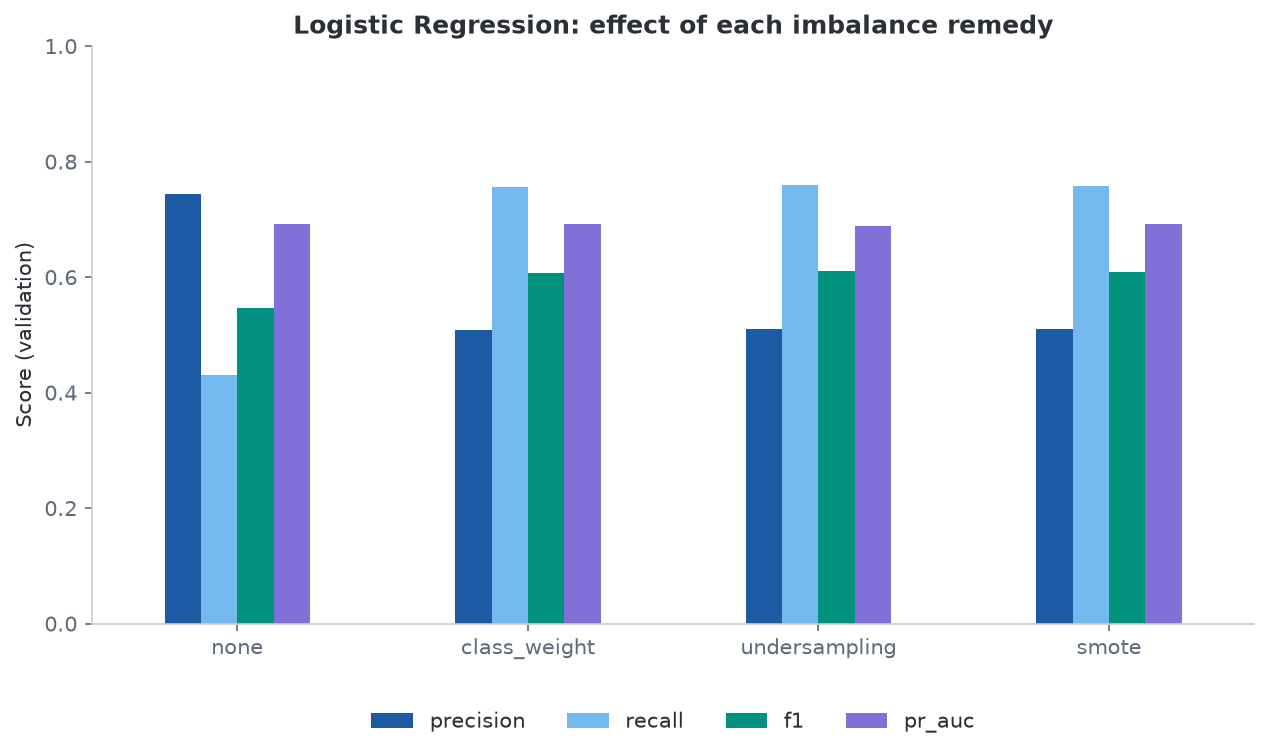
\includegraphics[width=\textwidth]{part2_01.png}
\caption{Class-imbalance remedies (validation).}
\end{subfigure}
\hfill
\begin{subfigure}{0.49\textwidth}
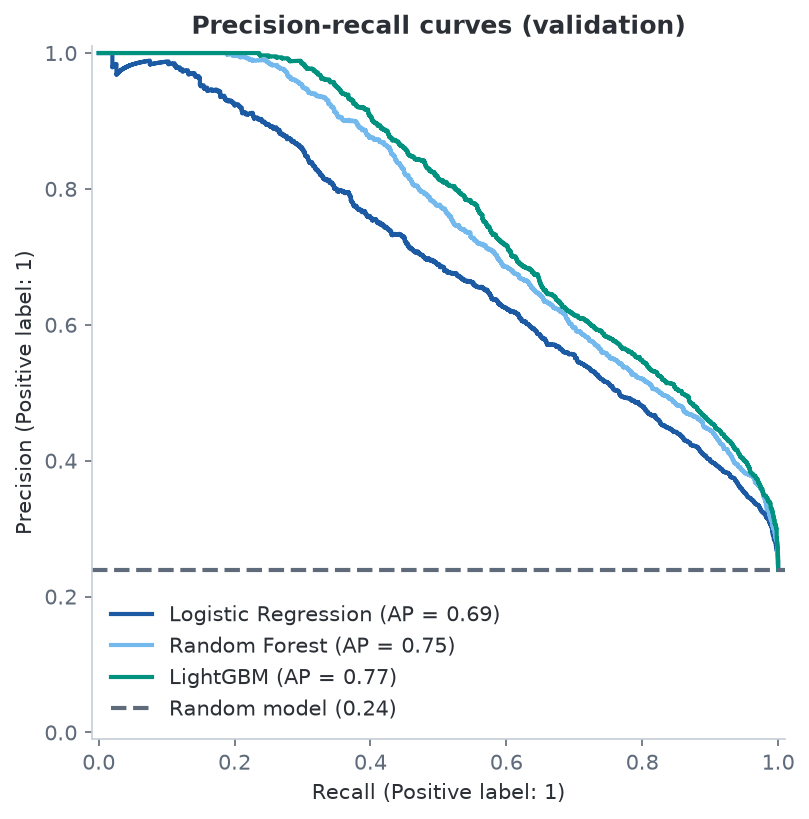
\includegraphics[width=\textwidth]{part2_03.png}
\caption{Precision-recall curves of the three models (validation).}
\end{subfigure}
\caption{Class-imbalance remedies and model comparison.}
\end{figure}

\begin{figure}[H]
\centering
\begin{subfigure}{0.49\textwidth}
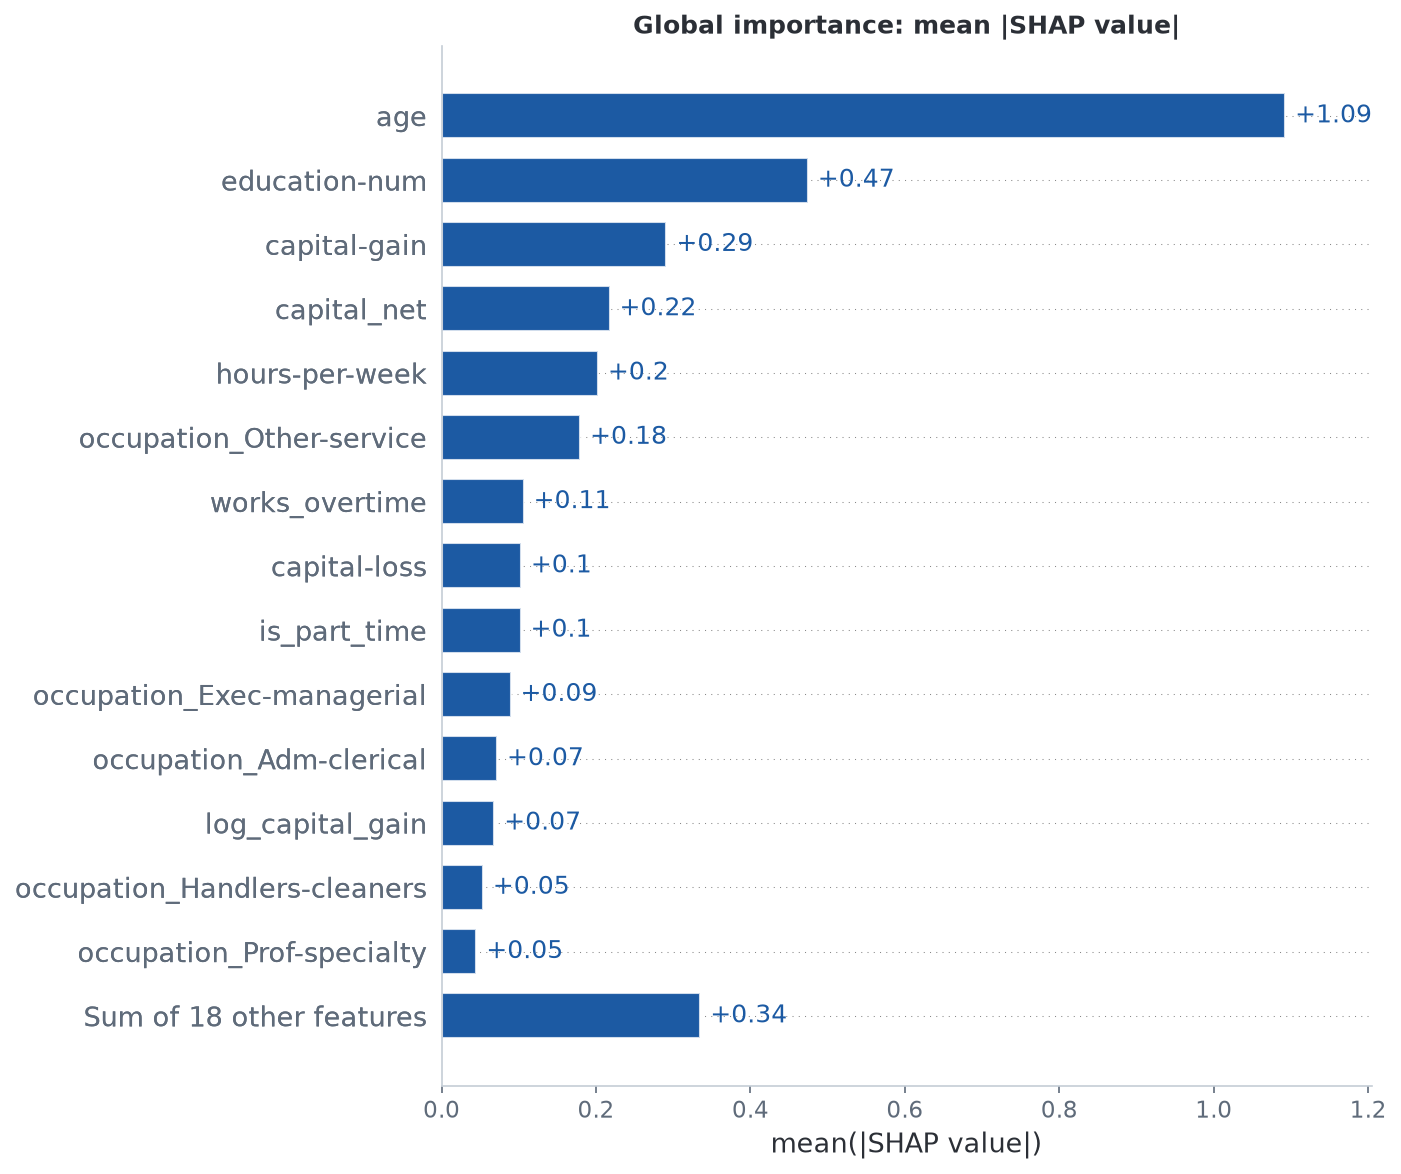
\includegraphics[width=\textwidth]{part4_01.png}
\caption{Mean $|$SHAP$|$ (global importance).}
\end{subfigure}
\hfill
\begin{subfigure}{0.49\textwidth}
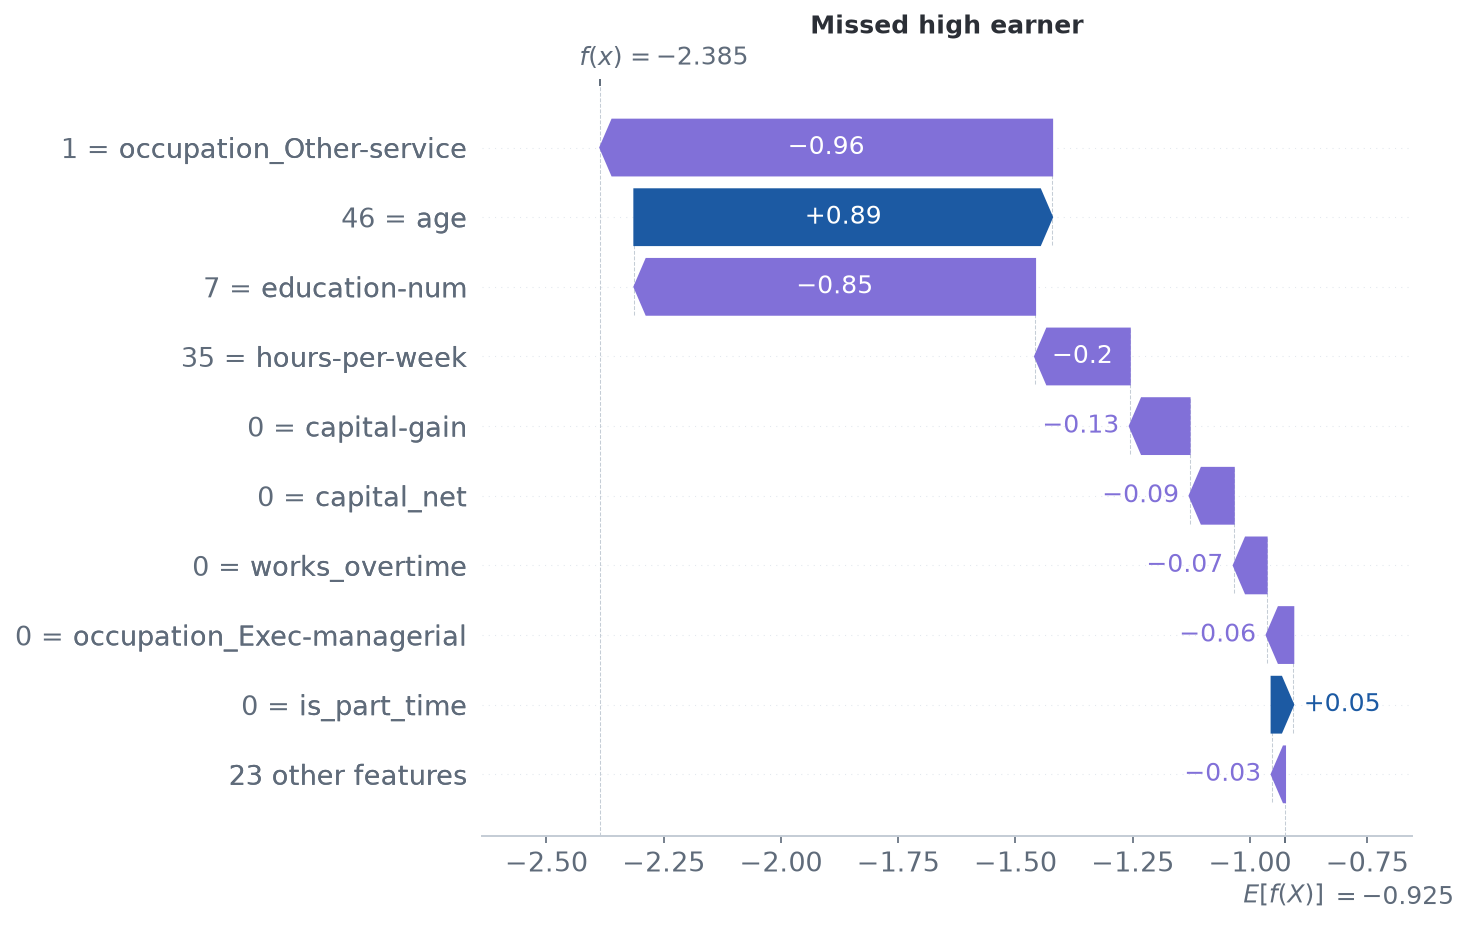
\includegraphics[width=\textwidth]{part4_05.png}
\caption{Missed high earner (really $>$50K, predicted 0.08).}
\end{subfigure}
\caption{Additional SHAP explanations.}
\end{figure}

\begin{figure}[H]
\centering
\begin{subfigure}{0.49\textwidth}
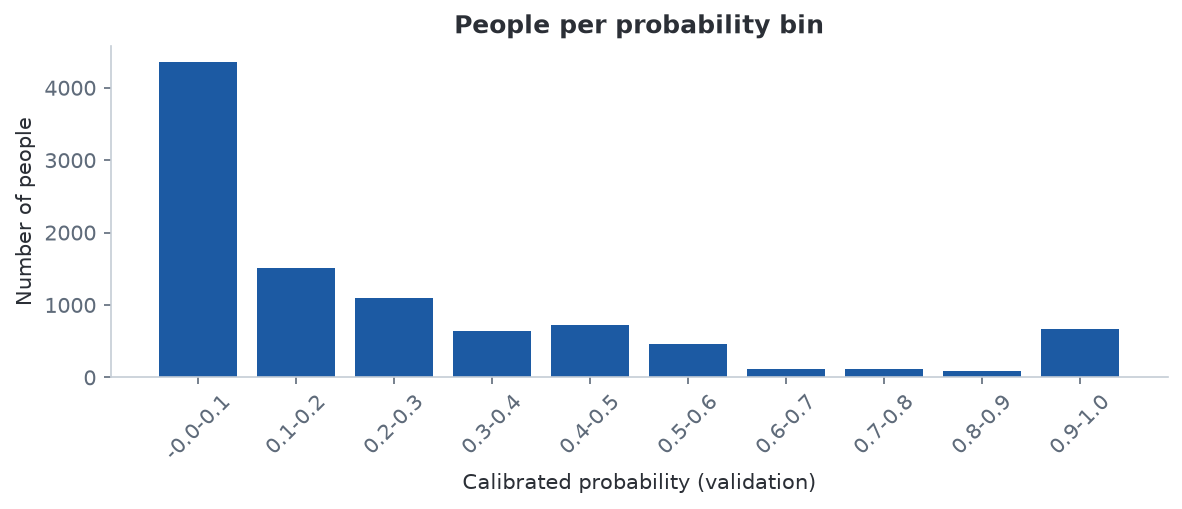
\includegraphics[width=\textwidth]{part4_09.png}
\caption{People per probability bin.}
\end{subfigure}
\hfill
\begin{subfigure}{0.49\textwidth}
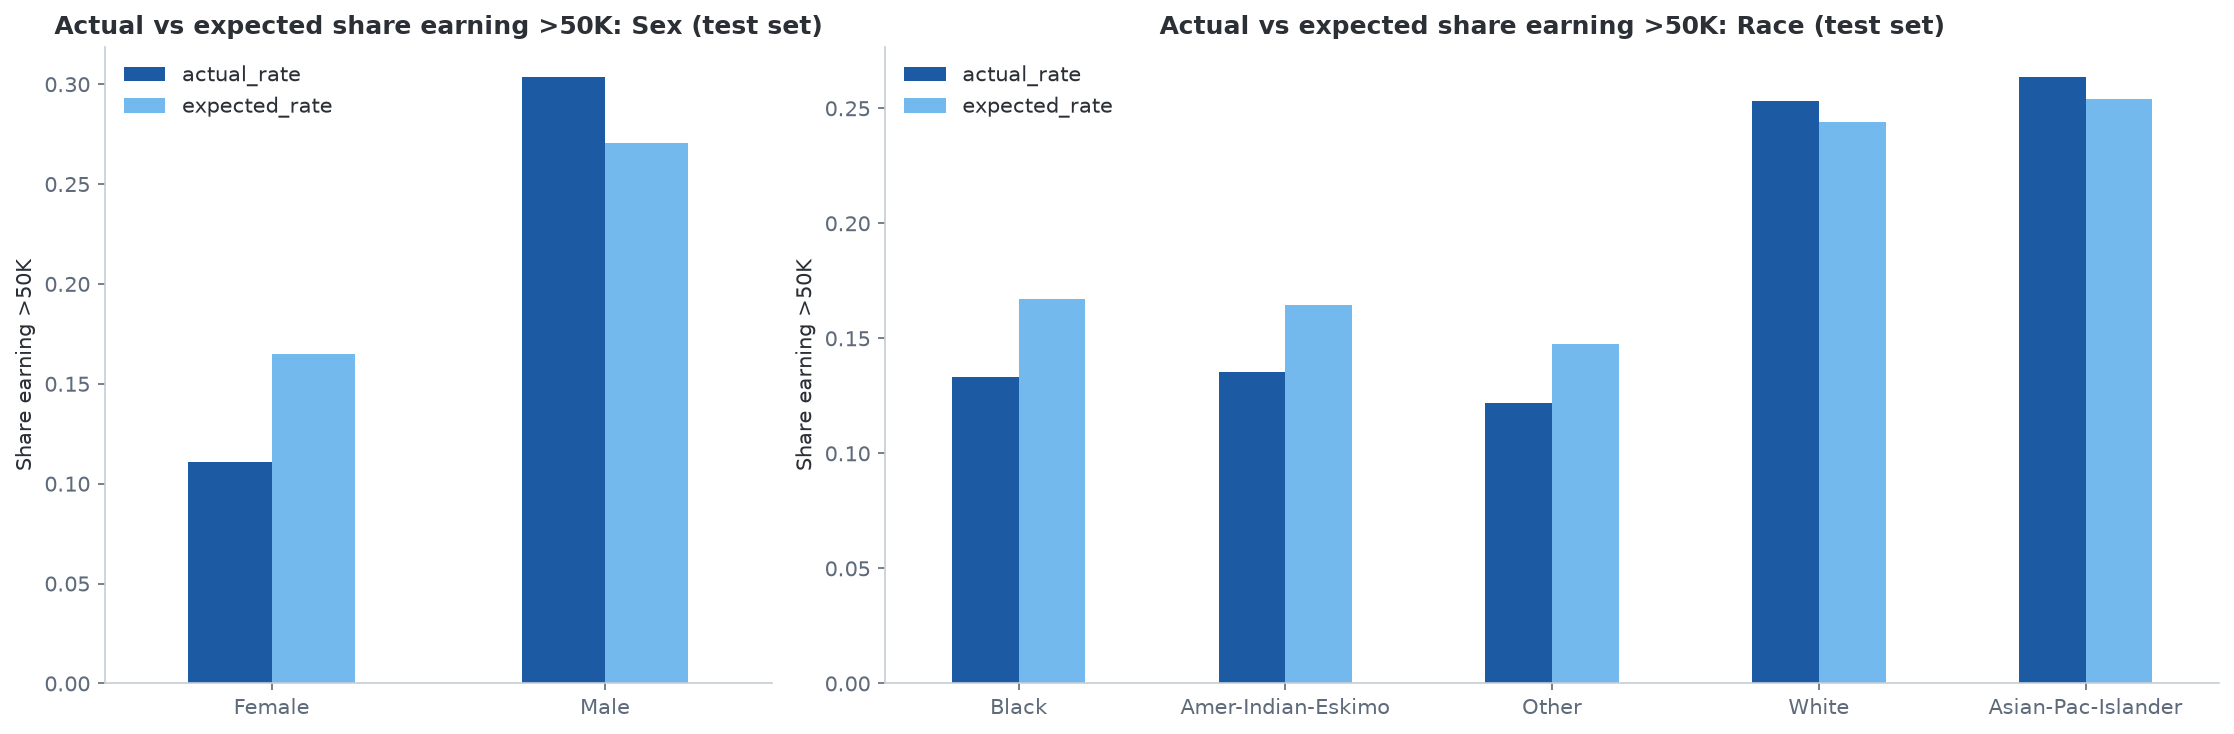
\includegraphics[width=\textwidth]{part4_12.png}
\caption{Actual vs expected rate by group.}
\end{subfigure}
\caption{Calibration support and audit rates (test set).}
\end{figure}

\begin{figure}[H]
\centering
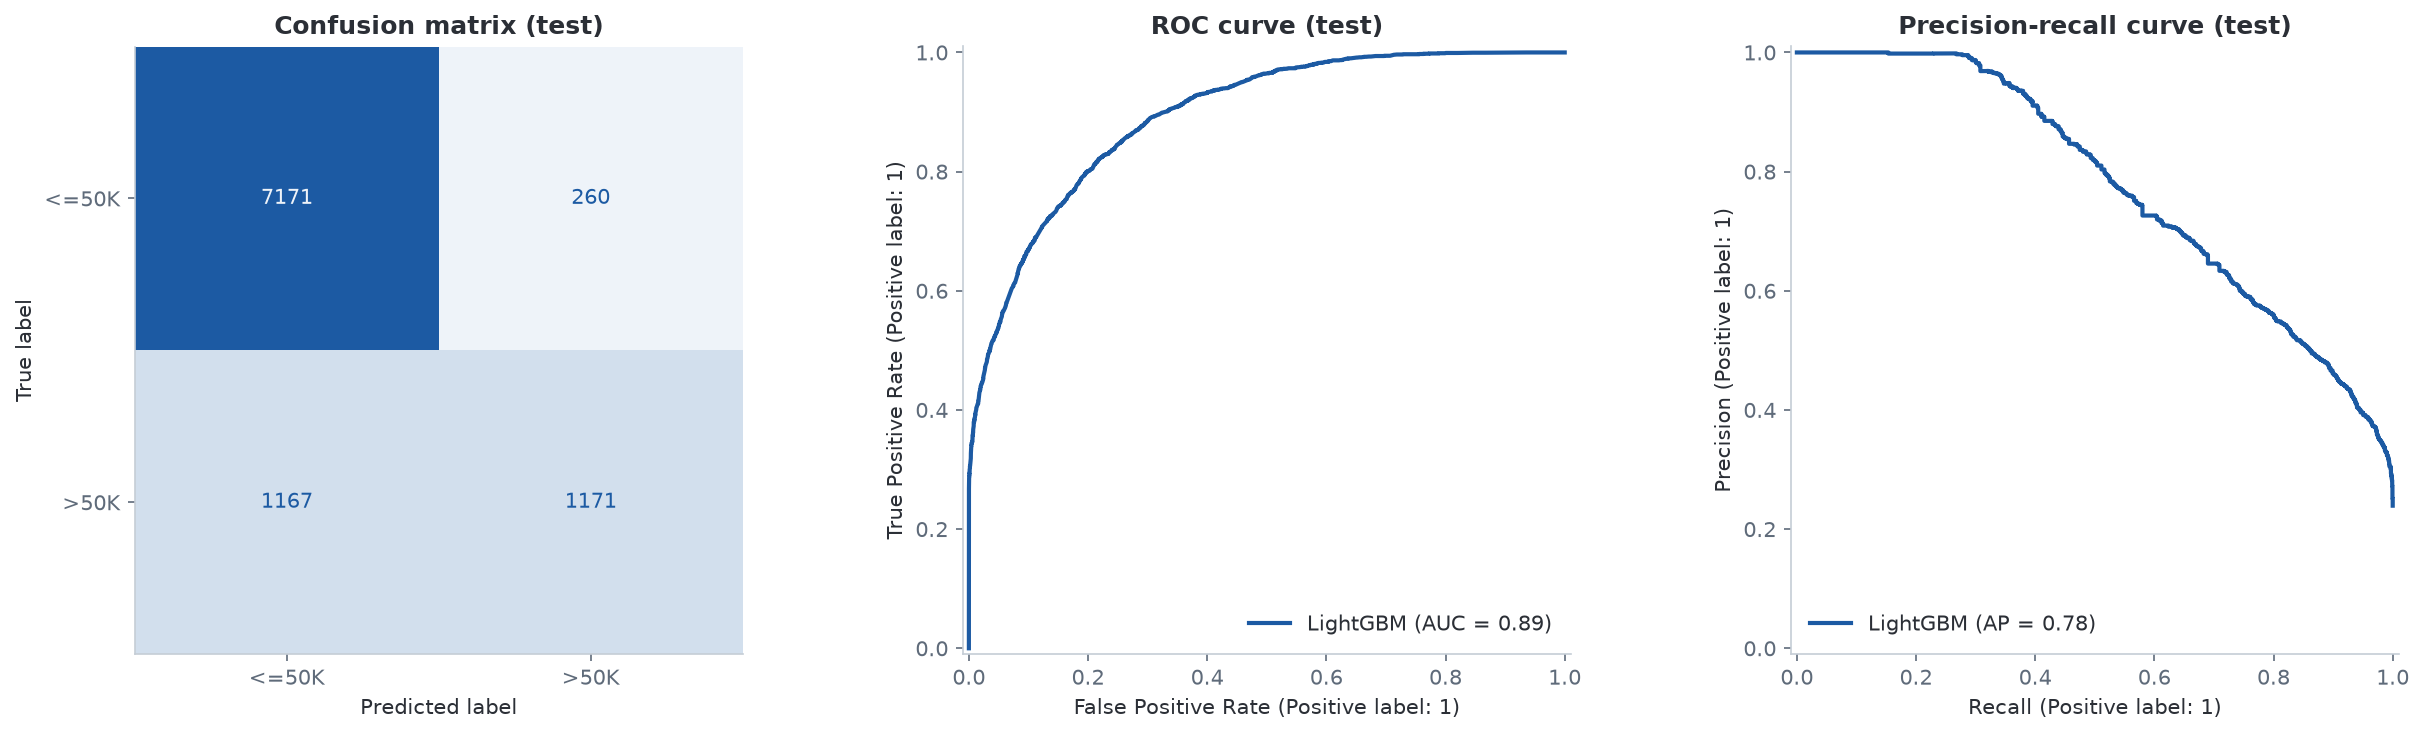
\includegraphics[width=\textwidth]{part4_11.png}
\caption{Final model on the test set: confusion matrix, ROC and precision-recall curves.}
\end{figure}

\begin{figure}[H]
\centering
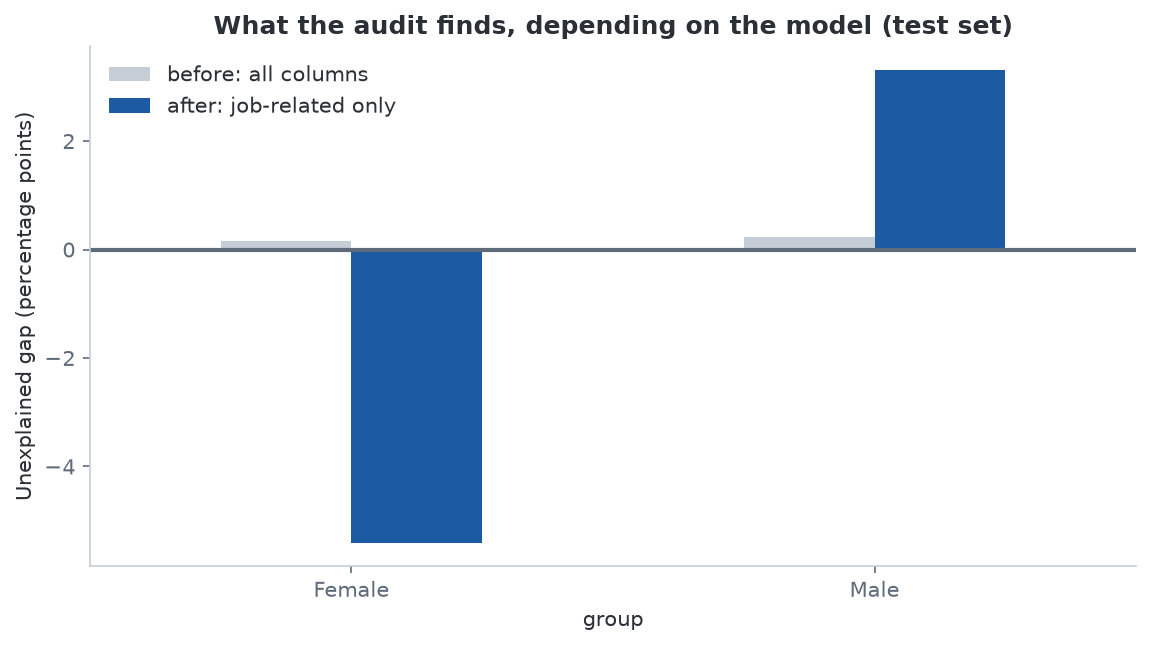
\includegraphics[width=0.7\textwidth]{part4_14.png}
\caption{Unexplained gap by sex before and after the mitigation (test set): the model trained on all columns finds no gap.}
\end{figure}

\end{document}
